\documentclass[14pt,a4paper]{article}
\usepackage[utf8]{inputenc}
\usepackage[russianb]{babel}
\usepackage[left=1.5cm,right=1.5cm,top=2cm,bottom=2.5cm]{geometry}
\usepackage{setspace}
\usepackage{indentfirst}
\usepackage{amssymb}
\usepackage{amsmath}
\usepackage{bm}

\usepackage{array}
\usepackage[pdftex]{graphicx}
\usepackage{comment}
\usepackage[table,xcdraw]{xcolor}


\usepackage{verbatim}


\graphicspath{{images/}}
\renewcommand{\baselinestretch}{1.3}

\begin{document}

Откроем файл таблицы. Скопируем таблицу ниже, но без чисел, оставив
только форматирование. В ячейку $A22$ скопируем значение ячейки $A1$.

\begin{center}
    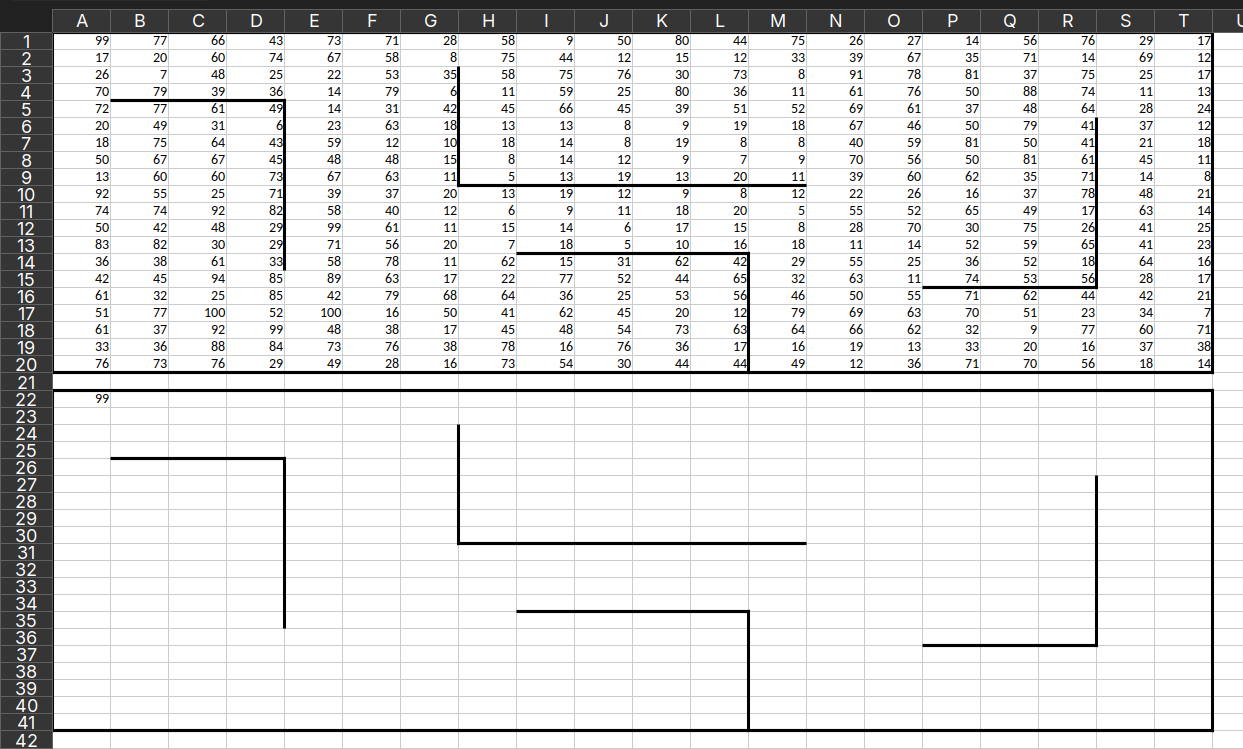
\includegraphics[width=0.5\textwidth]{1.png}
\end{center}

В ячейку $B22$ запишем формулу и растянем вправо до конца таблицы:
\begin{center}
    =B1+A22
\end{center}

В ячейку $A23$ запишем формулу и растянем вниз до конца таблицы:
\begin{center}
    =A2+A22
\end{center}

В ячейку B23 запишем формулу и растянем по оставшейся таблице:
\begin{center}
    =B2+МАКС(A23;B22)
\end{center}

\begin{center}
    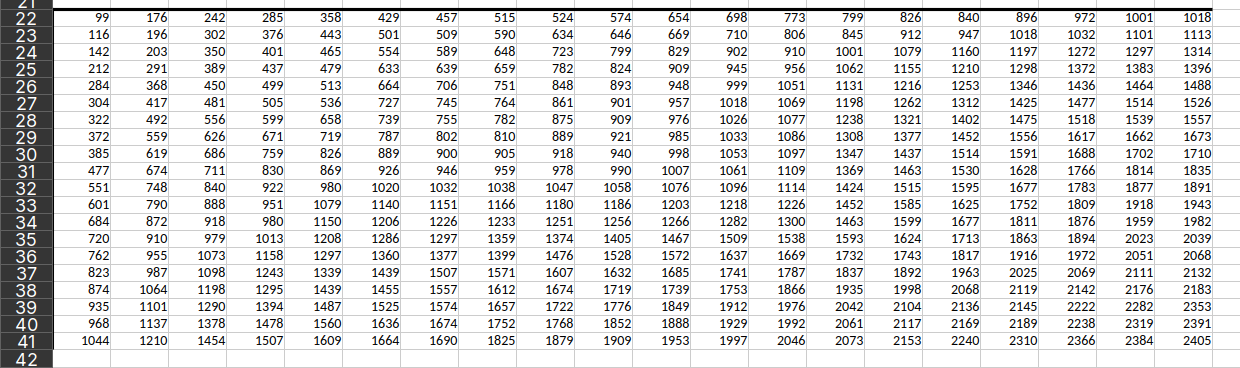
\includegraphics[width=0.5\textwidth]{2.png}
\end{center}

Стены пропали, поэтому необходимо снова скопировать форматирование с
верхней таблицы. В клетки под стеной можно попасть только командой
\textbf{вправо}, а в клетки справа от стены - командой \textbf{вниз}.

Отметим зелёным цветом клетки под стенками и синим -- клетки справа
от стенок. Также отметим красным <<угловые
клетки>> Скопируем в зелёные клетки формулу из $B22$, а в синие - из
$A23$.

\begin{center}
    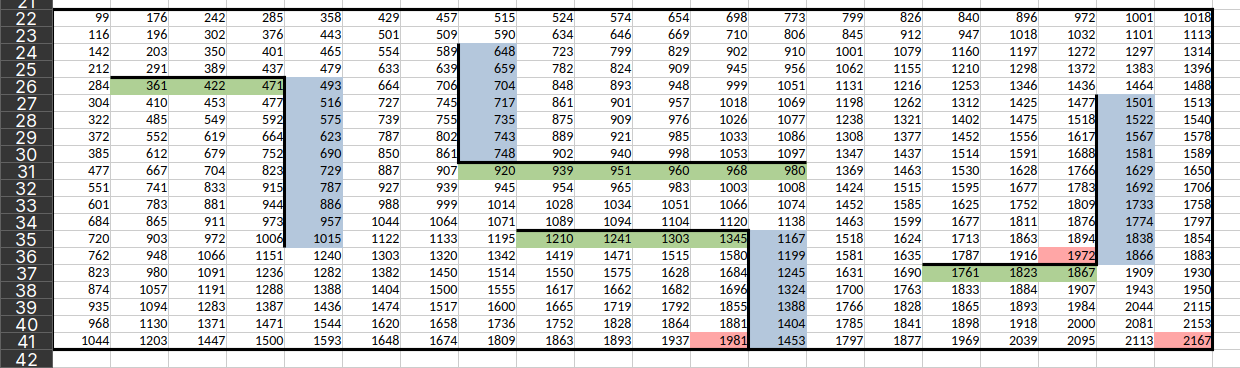
\includegraphics[width=0.5\textwidth]{3.png}
\end{center}

Из трёх красных клеток выбираем максимальную сумму 2167 -- это первый
ответ.

Для нахождения минимальной суммы, заменяем в таблице все МАКС на МИН
с помощью клавиш <<CTLR+H>>. Получаем 718.

\end{document}
